\documentclass{beamer}

\usepackage{amsmath}
\usepackage{mathdots}
\pagenumbering{arabic}
\usepackage{hyperref}
\usepackage{lscape}
\definecolor{slidetitlecolor}{RGB}{51,0,102}
\setbeamertemplate{footline}[frame number]%puts frame numbers in slide
\setbeamercolor{frametitle}{fg=slidetitlecolor}
\definecolor{item1color}{RGB}{51,153,255}
\setbeamercolor{itemize item}{fg=item1color}
\setbeamertemplate{itemize item}[circle]
\setbeamercolor{enumerate item}{fg=item1color}

\title{Markov Chains\vspace{-.5cm}}
\author{VK\\
Room: M1.30\\
\url{knightva@cf.ac.uk}\\
\url{www.vincent-knight.com}\\}
\date{\tiny{Last updated: \today.}}





\begin{document}

\maketitle


\frame{\frametitle{Markov Chains}
\tableofcontents
}

\section{Stochastic Processes and Markov Chains}

\frame{\frametitle{Stochastic Processes and Markov Chains}
}

\frame{\frametitle{Stochastic Processes}
\begin{itemize}
	\item It is often possible to represent the behaviour of a system by a collection of ``states''.
	\item The system being modelled is assumed to occupy one and only one state at any moment in time.
	\item The evolution of the system is represented by transitions from state to state.
\end{itemize}
}


\frame{\frametitle{Stochastic Processes}
An example of this could be the behaviour of the weather:\\

\begin{center}
	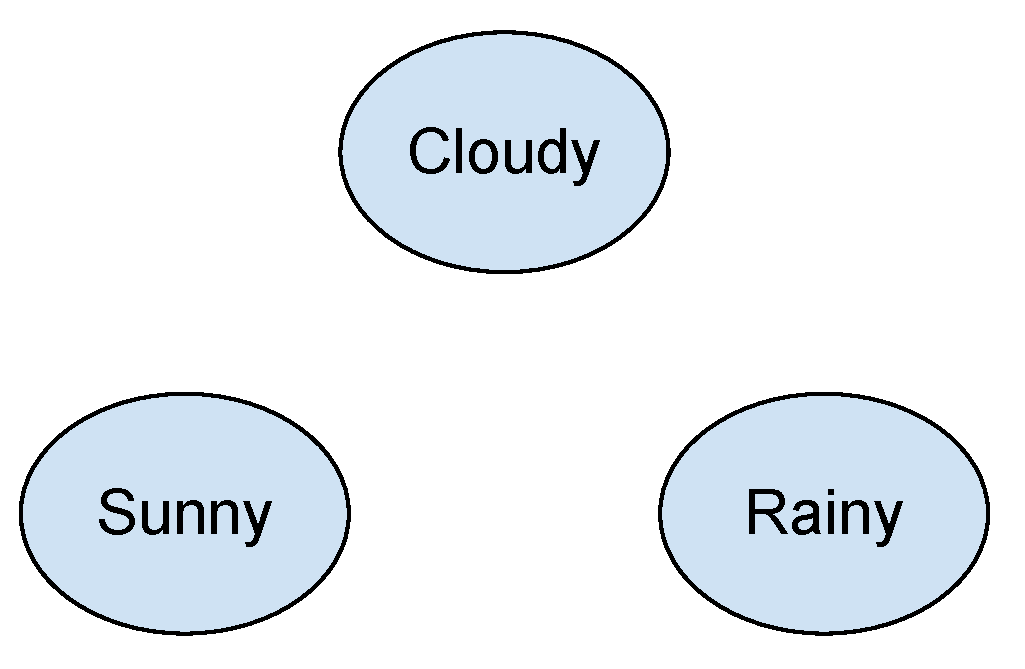
\includegraphics[width=8cm]{weather_states.pdf}
\end{center}
}

\frame{\frametitle{Formal definition of a Stochastic Process}
A stochastic process is defined as a family of random variables $\{X(t),\;t\in T\}$.\\

\begin{itemize}
	\item $T$ represents the index set.
	\begin{itemize}
		\item $T$ can be discrete: $T=\{0,1,2,3,...\}$: \emph{Discrete time stochastic process}.
		\item $T$ can be continuous: $T=\mathbb{R}_{\geq 0}$: \emph{Continuous time stochastic process}.
	\end{itemize}
	\item The values assumed by the random variables $X(t)$ are called states. The set of all possible values of $X(t)$ is called the state space: $\Omega$.
	\begin{itemize}
		\item $\Omega$ can be discrete: $\{\text{Rainy}, \text{Sunny}, \text{Cloudy}\}$
		\item $\Omega$ can also be continuous.
	\end{itemize}
\end{itemize}
}


\frame{\frametitle{Chains}
When $Omega$ is discrete, the stochastic process is called a \emph{chain}. For the rest of the course we will be concerned with:
\begin{center}
\emph{Homogeneous} Markov Chains.
\end{center}\pause

\begin{itemize}
	\item Discrete
	\item Continuous
\end{itemize}
}


\section{Discrete Markov Chains}

\frame{\frametitle{Discrete Markov Chains}
}

\frame{\frametitle{Definition of a Discrete Markov Chain}
For a discrete Markov chain we observe the state of a system at a discrete, but infinite set of times. We may take:
$$T=\mathbb{N}=\{0,1,2,\dots\}$$
The state of the system is then denoted as $X_0,X_1,X_2,\dots$. A discrete time Markov chain is then a stochastic process that satisfies the following relationship:

$$P(X_{n+1}=x_{n+1}|X_n=x_n,\dots,X_0=x_0)=P(X_{n+1}=x_{n+1}|X_n=x_n)$$
For ease of notation we write the probability of going from state $i$ to state $j$ at time period $n$ as:
$$p_{ij}(n)=P(X_{n+1}=j|X_n=i)$$
}


\frame{\frametitle{Transition Probability Matrix}

$$P(n)=
\begin{pmatrix}
p_{00}(n)&p_{01}(n)&p_{02}(n)&\dots&p_{0j}(n)&\dots\\
p_{20}(n)&p_{11}(n)&p_{12}(n)&\dots&p_{1j}(n)&\dots\\
p_{20}(n)&p_{21}(n)&p_{22}(n)&\dots&p_{2j}(n)&\dots\\
\vdots&\vdots&\vdots&\vdots&\vdots&\vdots\\
p_{i0}(n)&p_{i1}(n)&p_{i2}(n)&\dots&p_{ij}(n)&\dots\\
\vdots&\vdots&\vdots&\vdots&\vdots&\vdots
\end{pmatrix}
$$
$P(n)$ is a stochastic matrix:
\begin{itemize}
	\item $\sum_{j}p_{ij}(n)=1$ for all $i\in\Omega$
	\item $p_{ij}(n)\geq 0$ for all $i,j\in\Omega$
\end{itemize}
}

\frame{\frametitle{Homogeneous Markov Chains}
In a Homogeneous Markov Chain the transition rates do not depend on the amount of time that has passed:
$$P(k)=P(0)\text{ for all }k$$
This is what we consider in this course.
}

\frame{\frametitle{Weather Example}
This stochastic matrix:
$$\begin{pmatrix}
.2&.5&.3\\
.1&.1&.8\\
.1&.2&.7
\end{pmatrix}$$
corresponds to:
\begin{center}
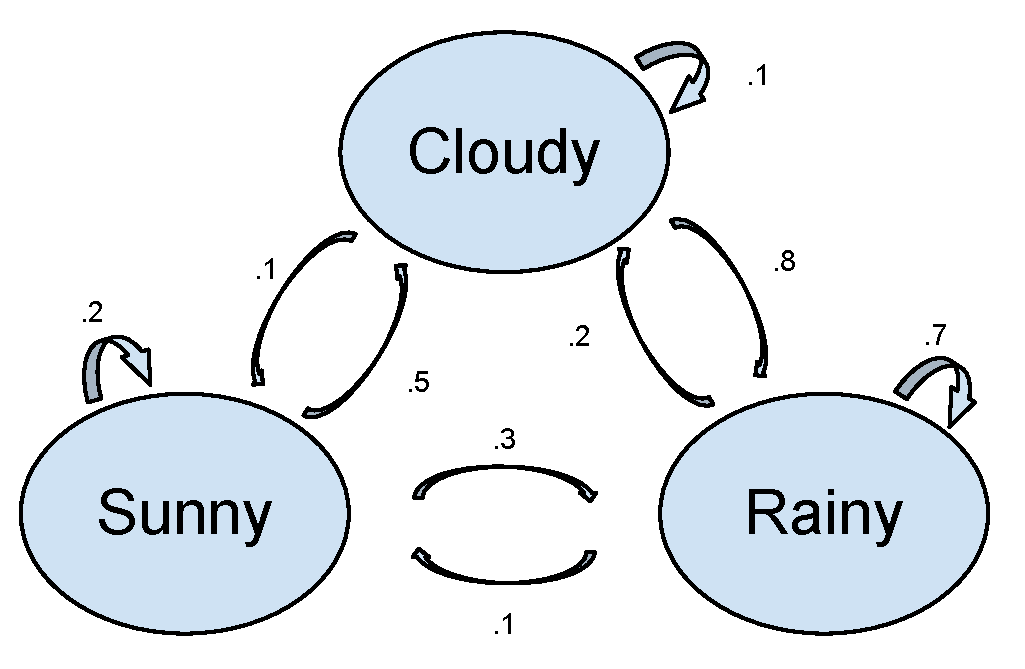
\includegraphics[width=8cm]{weather_chain.pdf}
\end{center}
}


\frame{\frametitle{State Vector}
We can describe the state of a Markov Chain by a vector: $\pi^{(n)}$. $\pi^{(n)}_j$ denotes the probability of being in State $j$ at time $n$:
\begin{itemize}
	\item $\sum_{j\in\Omega}\pi_{j}^{(n)}=1$ for all $n$
	\item $\pi_{j}^{(n)}\geq0$ for all $j,n$.
\end{itemize}
}

\frame{\frametitle{Weather example}
Assume $\pi^{(0)}=(1,0,0)$, what is $\pi^{(1)}$?
\begin{center}
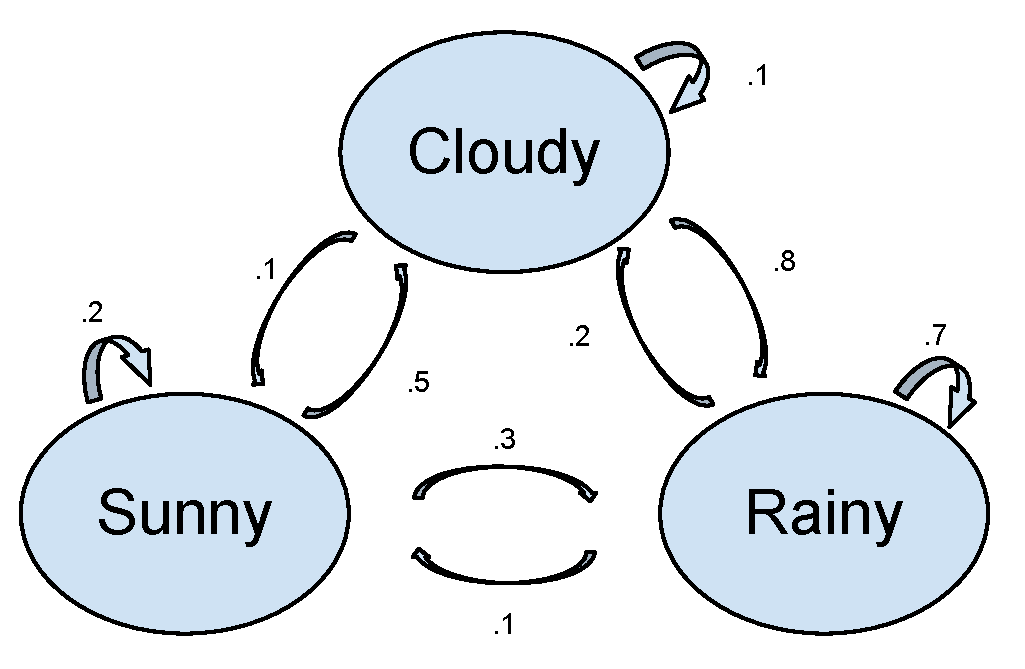
\includegraphics[width=8cm]{weather_chain.pdf}
\end{center}
\pause
$$\pi^{(1)}=(.2,.5,.3)$$
}


\frame{\frametitle{Powers of Transition Probability Matrix}
In general:
$$\pi^{(n+1)}=\pi^{(n)}P$$
Thus:
$$\pi^{(n)}=\pi^{(0)}P^n$$
}

\frame{\frametitle{Weather Example}
\only<1>{$$\pi^{(0)}=(1,0,0)$$\begin{center}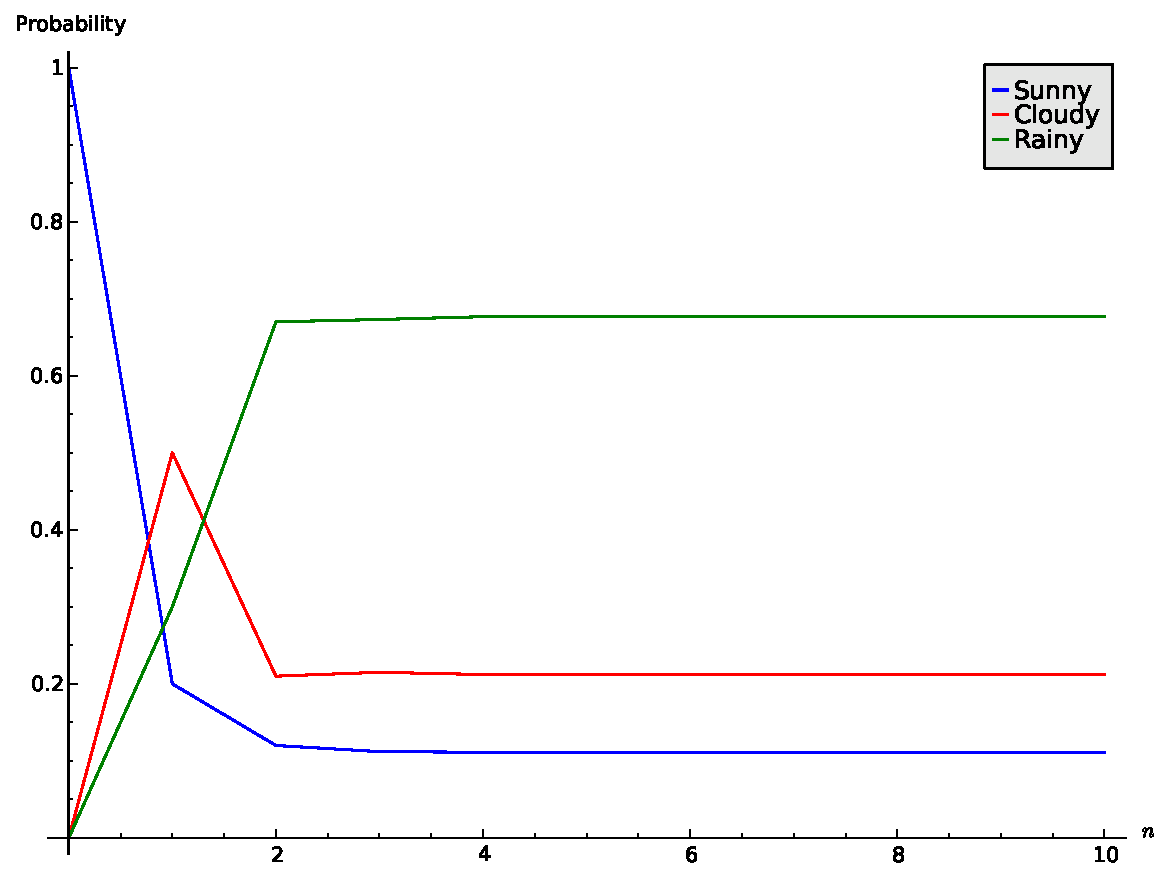
\includegraphics[width=10cm]{weather_probabilities-100.pdf}\end{center}}
\only<2>{$$\pi^{(0)}=(0,1,0)$$\begin{center}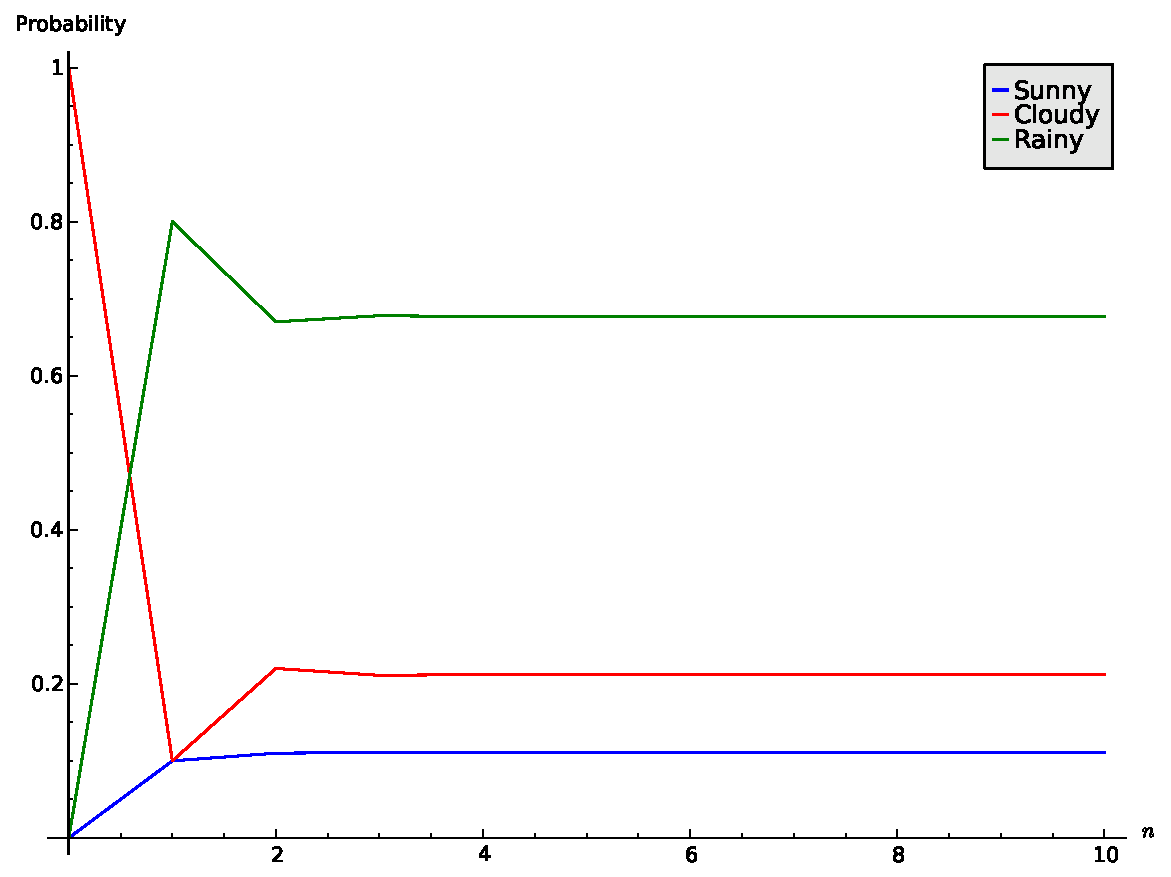
\includegraphics[width=10cm]{weather_probabilities-010.pdf}\end{center}}
\only<3>{$$\pi^{(0)}=(0,0,1)$$\begin{center}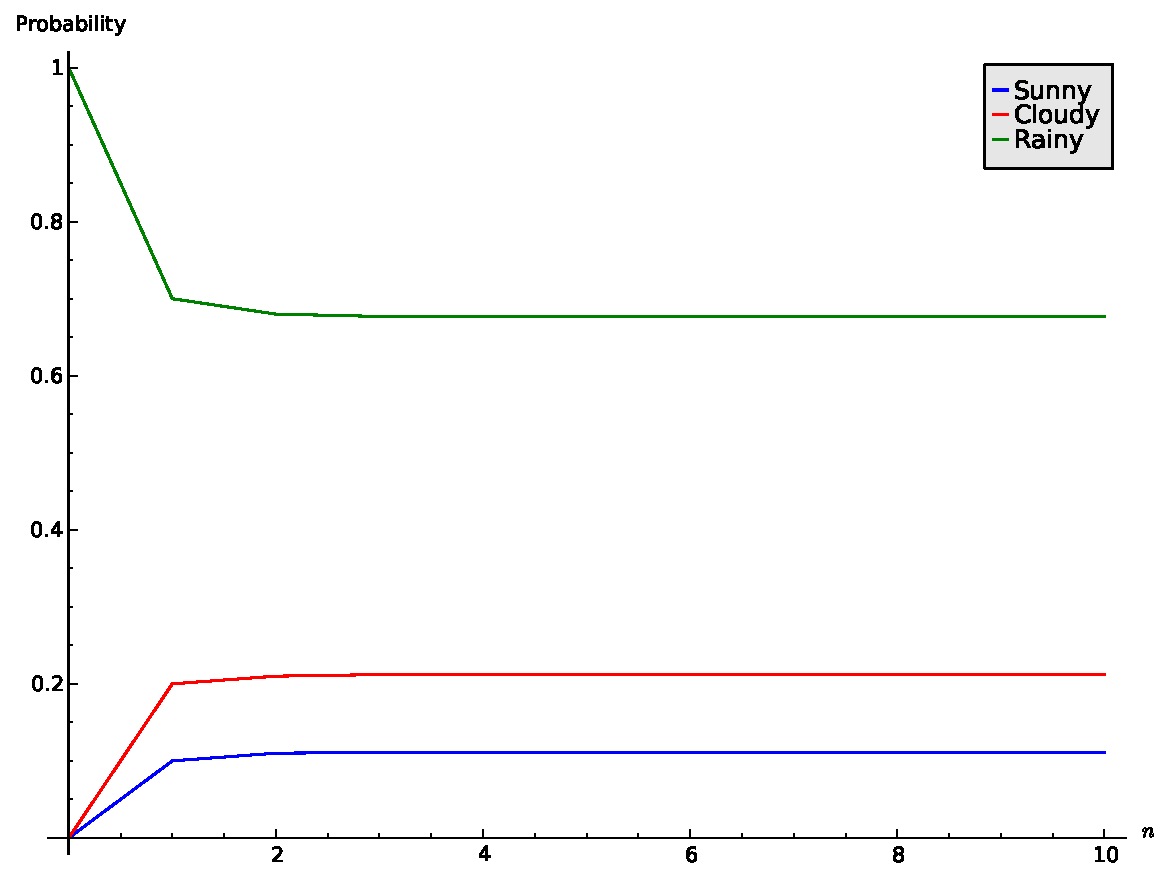
\includegraphics[width=10cm]{weather_probabilities-001.pdf}\end{center}}
\only<4>{$$\pi^{(0)}=(1/3,1/3,1/3)$$\begin{center}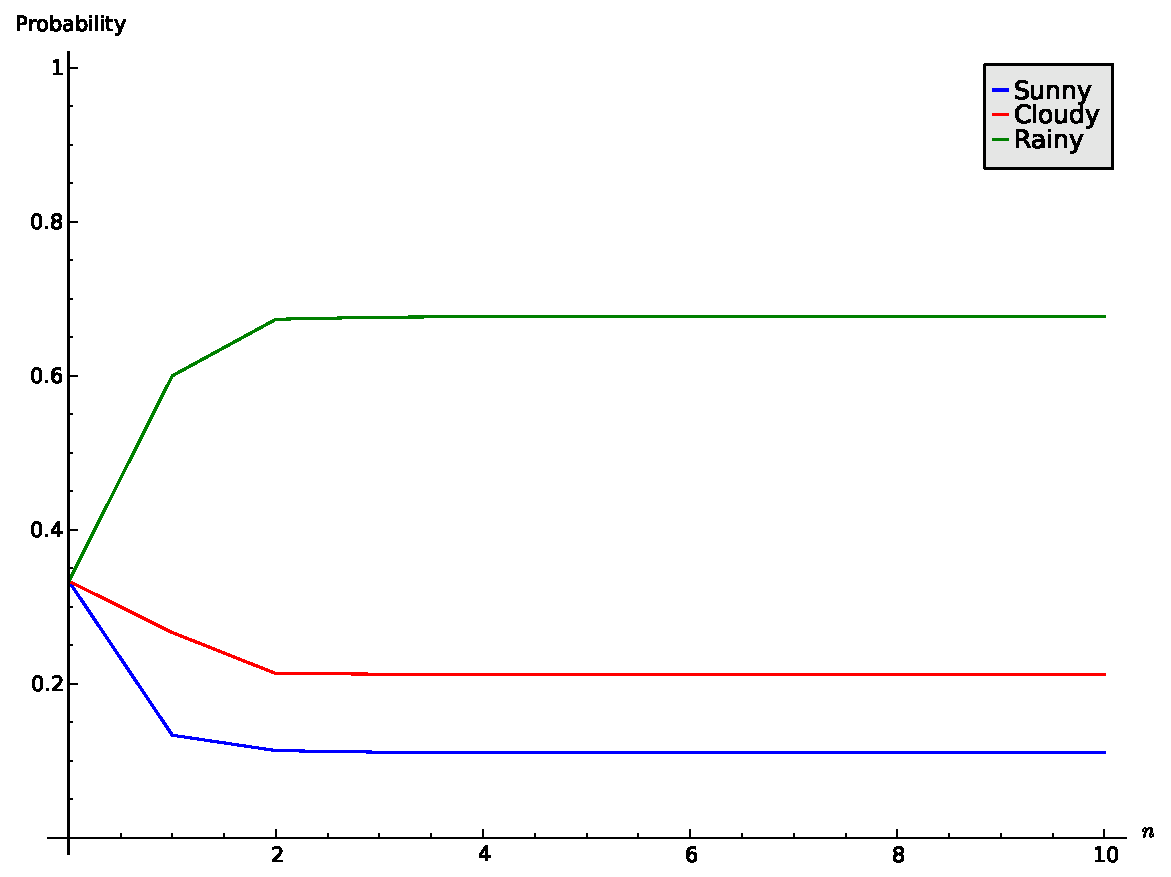
\includegraphics[width=10cm]{weather_probabilities-333.pdf}\end{center}}
\only<5>{$$\pi^{(0)}=(.25,.25,5)$$\begin{center}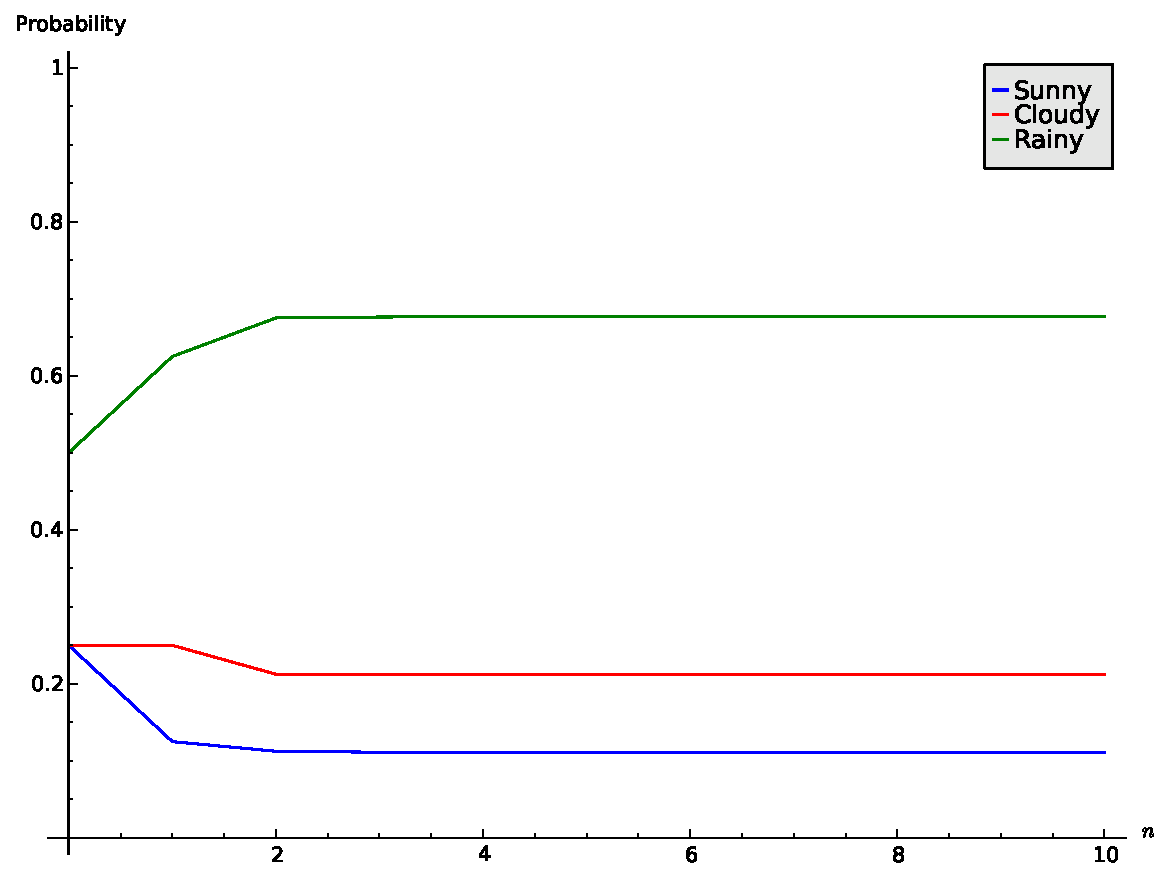
\includegraphics[width=10cm]{weather_probabilities-25.pdf}\end{center}}
}

\frame{\frametitle{Limiting and Steady State Distribution}
\begin{itemize}
	\item If the limit:
$$\lim_{n\to\infty}P^{n}$$
exists, then the probability distribution $\pi=\lim_{n\to\infty}\pi^{(0)}P^n$ is called the limiting distribution. (Note that this can depend on $\pi^{(0)}$).
	\item If a limiting distribution exists and it is independent of $\pi^{(0)}$ it is called a steady state distribution. Such a distribution satisfies:
$$\pi=\pi P$$
\end{itemize}
}

\frame{\frametitle{Weather Example}
$$\pi=\pi P\Rightarrow\begin{cases}
\pi_1=.2\pi_1+.1\pi_2+.1\pi_3\\
\pi_2=.5\pi_1+.1\pi_2+.2\pi_3\\
\pi_3=.3\pi_1+.8\pi_2+.7\pi_3
\end{cases}$$
Solving this gives:
$$\begin{cases}
\pi_1={11\over 67}c\\
\pi_2={21\over 67}c\\
\pi_3=c
\end{cases}$$
For some $c$. Recalling that $\pi_1+\pi_2+\pi_3=1$ gives:
$$\begin{cases}
\pi_1={1\over 9}\approx.11\\
\pi_2={7\over 33}\approx.21\\
\pi_3={67\over 99}\approx.68
\end{cases}$$
}

\section{Continuous Markov Chains}
\frame{\frametitle{Continuous Markov Chains}}

\frame{\frametitle{Transition Matrix}}

\frame{\frametitle{Exponent of a matrix}}

\frame{\frametitle{Steady state equation}}

\frame{\frametitle{Equivalence of Continuous and Discrete Markov Chains}}

\end{document}
